\documentclass[11pt,a4paper]{article}
\usepackage[top=.75in, bottom=.75in, left=1 in, right=1in]{geometry}
\usepackage{graphicx}
\usepackage{natbib}
\usepackage{gensymb}
%\begin{footnotesize}
%\address{1300 Centre Street \\ Boston, MA, 20131}
%\end{footnotesize}
\begin{document}
\bibliographystyle{..//refs/styles/besjournals.bst}
\def\labelitemi{--}
\parindent=24pt
\includegraphics[width=0.3\textwidth]{/Users/danielbuonaiuto/Desktop/arb_logo.png}
\pagenumbering{gobble}
\\\\
{Dear Dr. Hetherington,}\\

\noindent We propose a ``Viewpoint" about the drivers of flower-leaf phenological sequences (FLSs) in deciduous woody plants. Evolutionary theory predicts that both flowering and leaf phenology are critical fitness components of woody plants, and a century of empirical research supports this assertion \citep{Munguia-Rosas2011,Forrest2010}. In recent decades, this body of theory has been extended to suggest that it is not only individual phenophases but also the relationship between them that determines woody plant fitness \citep{Menzel1999,Ettinger2018}. Many deciduous woody plants flower before leafing, yet sustained research efforts have yet to yield a well-supported explanation for this. These unresolved hypotheses are critically important now as climate change is shifting FLSs--which may exacerbate fitness differences between species and reshape eco-systems of the future. Our ``Viewpoint" shows how progress in this area has been stalled by our conceptual framework for FLSs; we detail a new approach built on continuous measures of FLS and intra-specific and within-individual-level variation to rapidly advance progress.\\

\noindent \emph{What hypotheses or questions does this work address?}\\

\noindent Flowering before leafing may be an adaptation for wind-pollination \citep{Rathcke_1985}, reducing water stress \citep{Reich1984}, or early season flowering \citep{Primack1987}. Direct comparisons of these hypotheses are rare but tend to find support for more than one \citep{Gougherty2018,Bolmgren2003}. A novel approach focusing on intra-specific FLS variation and quantitative comparisons is necessary to accurately evaluate these hypotheses.\\

\noindent \emph{How does this work advance our current understanding of plant science?}\\

\noindent We show: 1) There is substantial inter- and intra- specific variation in FLS that cannot be accommodated in the current framework. 2) Variation provides novel insights about the function of FLSs, revealing consistencies and anomalies in support for the hypotheses. 3) Leveraging intra-specific variation will advance our understanding of FLS.\\

\noindent \emph{Why is this work important and timely?}\\

\noindent Climate change is altering FLSs, but effects vary across species and populations (Fig. \ref{fig:Figure 1}). Shifts could be beneficial or disastrous depending on the function of FLSs. Predicting this requires researchers to effectively evaluate current hypotheses. Our framework is the first that can do this, making it critical to fundamental and applied research.\\

 \noindent We expect this manuscript will be titled ``Reconciling competing hypotheses regarding flower-leaf sequences in temperate forests for fundamental and global change biology". It will be co-authored by I. Morales-Castilla, and E.M. Wolkovich. This proposed manuscript is not under consideration anywhere else. Thank you for your consideration.\\
\\Sincerely,\\

Daniel Buonaiuto
\newpage
\section*{Abstract:}
Phenology is a major component of organism fitness. It is not only individual phenological events that affect fitness, but also the relationship between events. Deciduous woody plants exhibit considerable variation in the order of reproductive and vegetative events, or flower-leaf sequences (FLSs). Research suggests that FLSs are adaptive, and several competing hypotheses may explain their function. Reconciling these hypotheses has been impeded by our conceptual orientation towards them. Classically, FLSs are treated categorically at the species level, obscuring substantial inter- and intra-specific variation. We develop the existing hypotheses to account for the FLS variation in nature and evaluate them with four case studies. Our inquiry provides major insights towards a new framework for understanding FLSs. First, we find concurrent support for multiple hypotheses. Future research should allow for overlapping hypotheses and test them in smaller sub-groupings. Second, support for FLS hypotheses is sensitive to how FLSs are defined. Researchers should switch from categorical to continuous measures of FLS. Finally, we highlight the limits of inter-specific trait-association models for hypothesis testing. Researchers should adopt an intra-specific approach and evaluate fitness consequences of FLS variation to test the FLS hypotheses and to predict how climate-related alterations to FLSs will affect plant communities.
\section*{Selected Figures:}
   \begin{figure}[ht!]
   \centering
 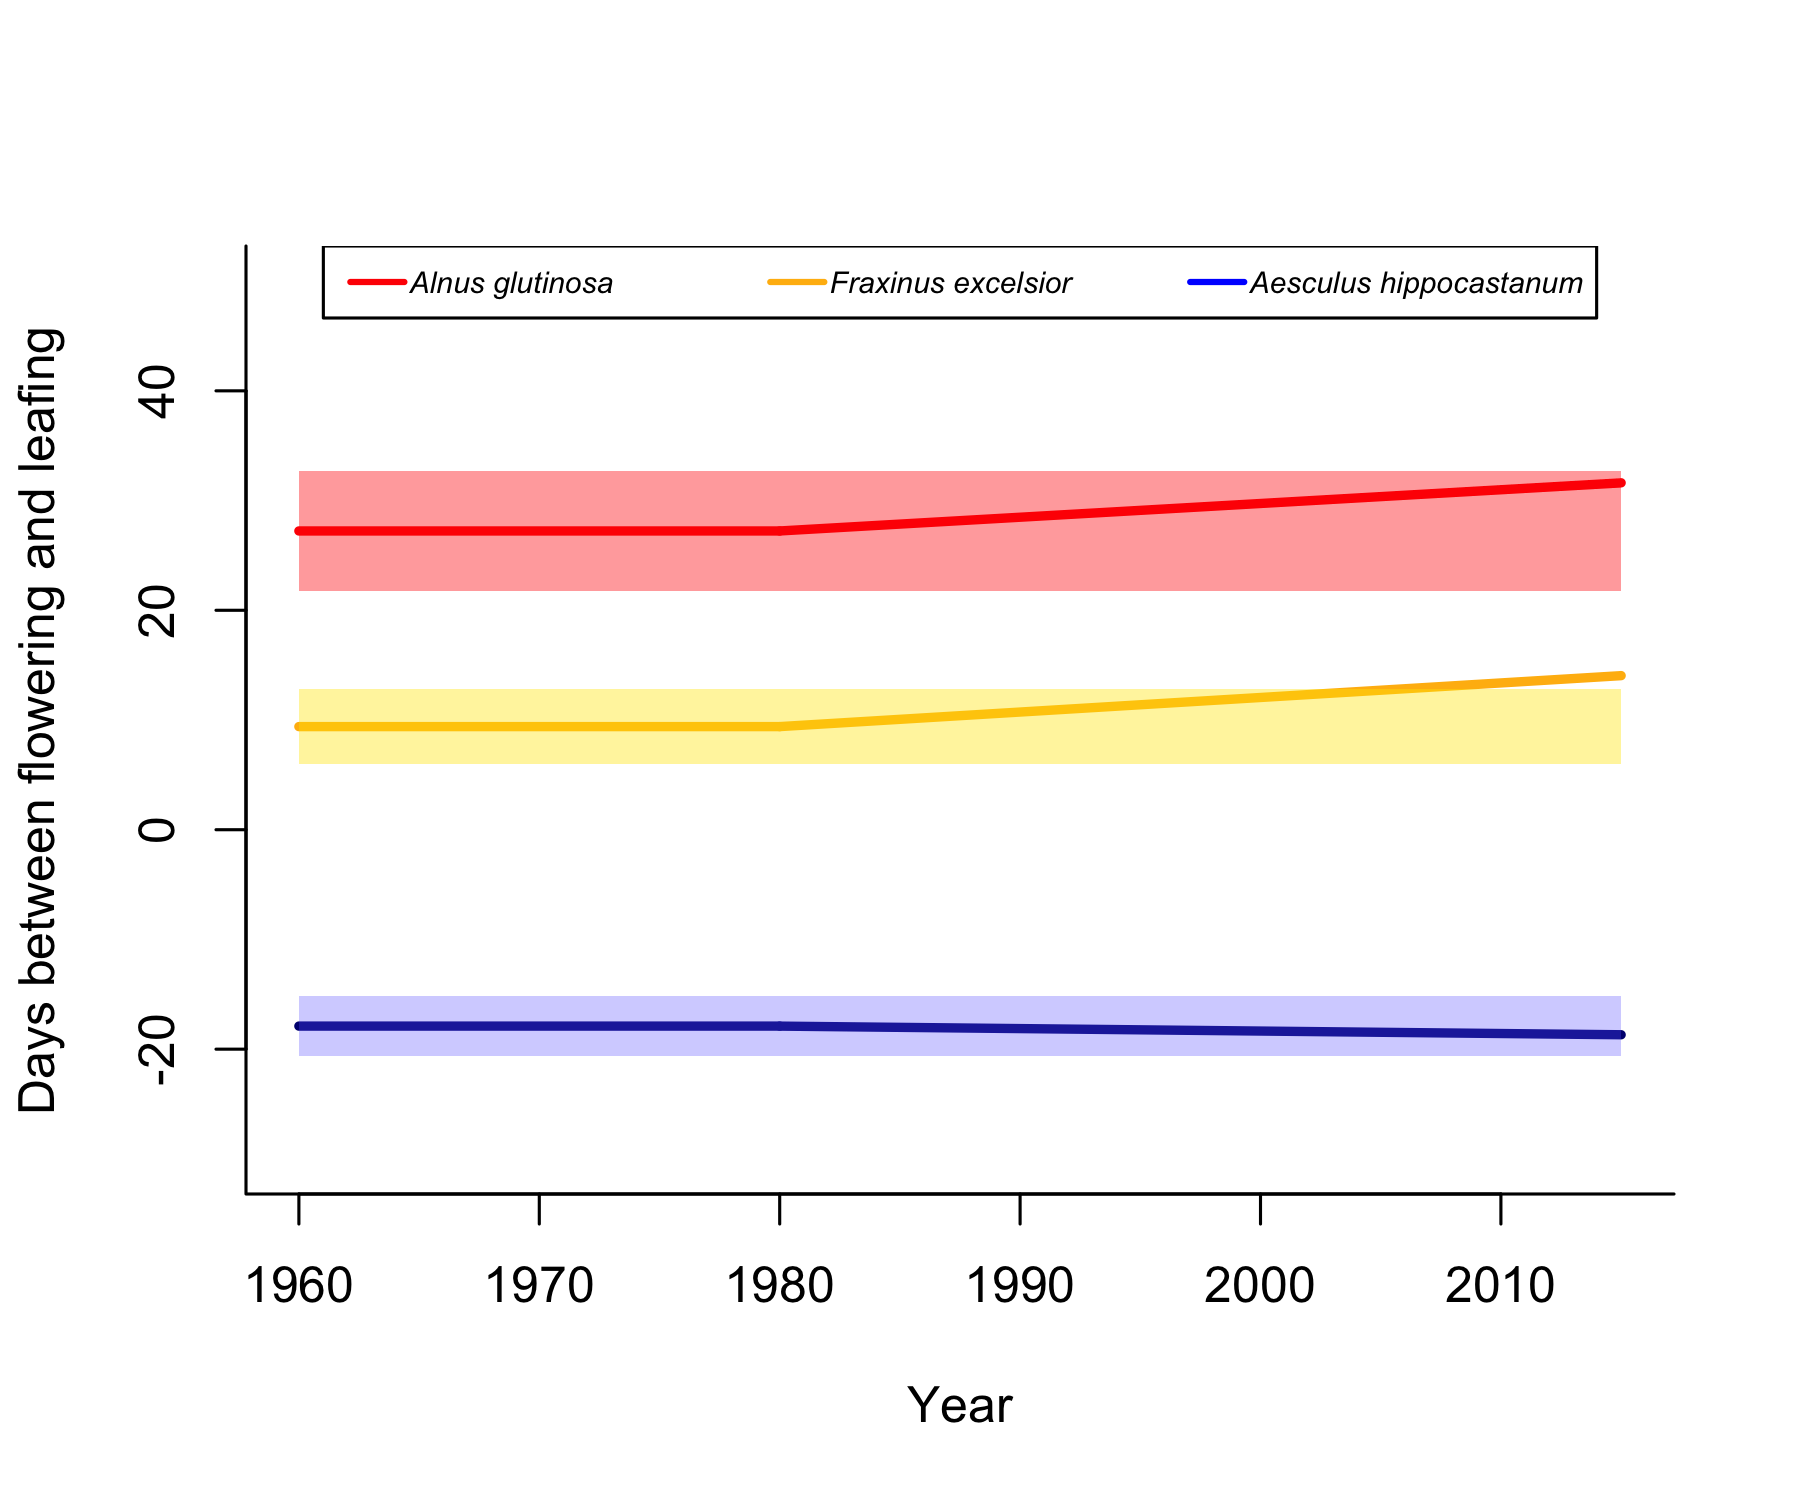
\includegraphics[width=.6\textwidth]{..//figure/FLS_climate_change.png}\\
\caption{\textbf{Modeled FLS response to climate change across Europe for three tree species from 1960 to 2015.} To detect the effect of climate change on average FLS, the models allows for shifts in FLS after 1980. Each small line represents a population from the PEP725 database while thicker lines represent the mean trend per species and the highlighted regions indicate historic range of FLS variability (upper and lower 95\% credible intervals of the pre-1980 average). There is significant intra-specific variation in average FLS and the FLS response to climate change. For all species, the time between flowering and leafing is generally increasing but the direction and rate of change differs across species and sites which may exacerbate fitness differences between species and communities.}
    \label{fig:Figure 1}
    \end{figure}
\newpage
\bibliography{..//refs/hyst_outline.bib}

\end{document}